
\section{Choose of tool for verification}
Software unit testing can achieved by almost any tool. This since its just more
or less about unit testing. This phase is hence not the most interesting when it
comes to the choose of a tool verification. Of course one can take the simplicity
to achieve good unit testing into account but still it is not what makes
a verification tool especially unique for the project goals.

Since the purposes is about benchmarking the software the phase ''verification of
software safety requirements'' will not influence the choose. For be able to test
this phase a greater amount of components of the hole system must be available. Such
components may include hardware etcetera. Implementation wise should everything
be able to run on a standard PC-machine.

The most interesting part is the software integration and testing. Is there a
tool that one can use to easily combine test and requirements from different
modules? Is it possible to test functional safety concept from this
combination, for example corrupting some software elements?

\subsection{Why QuickCheck and Erlang?}

\section{Specification}
Specifications for what each module should do in AUTOSAR is given in text form.
Hence one must first, before a module can be tested, implement the specification
for that module in code.
\section{Testing}
Properties for a module have to take the current state in consideration since
most functions written in an imperative language are not immutable. This gives
raise to the idea of an state machine based testing tool.
\begin{itemize}
\item Choose a specification which will be translated to QuickCheck properties
in parts.
\item With the use of statistics and confidence intervals, show that, with
enough tests the state-space will be exhausted.
\item Evaluate other semi-formal techniques and show that the results from them
shows that QuickCheck is reliable for verification.
\item Generalize the technique.
\end{itemize}


\section{Implementation}
A challenging step is the analysing part. If the testing tool returns zero
errors what does that say about the robustness of the input byte code? Passed
100 of 100 tests is just a statement and does not say anything more than that
some tests passed. Can tests be implemented in a clever way so that it is
possible to get some kind of confidence interval on the correctness of the code?
\begin{figure}[!ht]
% Graphic for TeX using PGF
% Title: /home/oskar/documents/box.dia
% Creator: Dia v0.97.2
% CreationDate: Sat Sep  7 19:28:43 2013
% For: oskar
% \usepackage{tikz}
% The following commands are not supported in PSTricks at present
% We define them conditionally, so when they are implemented,
% this pgf file will use them.
\ifx\du\undefined
  \newlength{\du}
\fi
\setlength{\du}{15\unitlength}
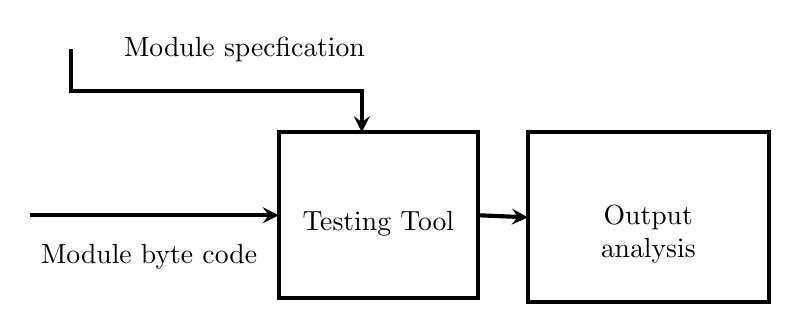
\begin{tikzpicture}
\pgftransformxscale{1.000000}
\pgftransformyscale{-1.000000}
\definecolor{dialinecolor}{rgb}{0.000000, 0.000000, 0.000000}
\pgfsetstrokecolor{dialinecolor}
\definecolor{dialinecolor}{rgb}{1.000000, 1.000000, 1.000000}
\pgfsetfillcolor{dialinecolor}
\definecolor{dialinecolor}{rgb}{1.000000, 1.000000, 1.000000}
\pgfsetfillcolor{dialinecolor}
\fill (6.000000\du,7.000000\du)--(6.000000\du,11.000000\du)--(10.795000\du,11.000000\du)--(10.795000\du,7.000000\du)--cycle;
\pgfsetlinewidth{0.100000\du}
\pgfsetdash{}{0pt}
\pgfsetdash{}{0pt}
\pgfsetmiterjoin
\definecolor{dialinecolor}{rgb}{0.000000, 0.000000, 0.000000}
\pgfsetstrokecolor{dialinecolor}
\draw (6.000000\du,7.000000\du)--(6.000000\du,11.000000\du)--(10.795000\du,11.000000\du)--(10.795000\du,7.000000\du)--cycle;
% setfont left to latex
\definecolor{dialinecolor}{rgb}{0.000000, 0.000000, 0.000000}
\pgfsetstrokecolor{dialinecolor}
\node at (8.397500\du,9.195000\du){Testing Tool};
\pgfsetlinewidth{0.100000\du}
\pgfsetdash{}{0pt}
\pgfsetdash{}{0pt}
\pgfsetbuttcap
{
\definecolor{dialinecolor}{rgb}{0.000000, 0.000000, 0.000000}
\pgfsetfillcolor{dialinecolor}
% was here!!!
\pgfsetarrowsend{stealth}
\definecolor{dialinecolor}{rgb}{0.000000, 0.000000, 0.000000}
\pgfsetstrokecolor{dialinecolor}
\draw (10.795000\du,9.000000\du)--(12.000000\du,9.050000\du);
}
\pgfsetlinewidth{0.100000\du}
\pgfsetdash{}{0pt}
\pgfsetdash{}{0pt}
\pgfsetbuttcap
{
\definecolor{dialinecolor}{rgb}{0.000000, 0.000000, 0.000000}
\pgfsetfillcolor{dialinecolor}
% was here!!!
\pgfsetarrowsend{stealth}
\definecolor{dialinecolor}{rgb}{0.000000, 0.000000, 0.000000}
\pgfsetstrokecolor{dialinecolor}
\draw (0.000000\du,9.000000\du)--(6.000000\du,9.000000\du);
}
% setfont left to latex
\definecolor{dialinecolor}{rgb}{0.000000, 0.000000, 0.000000}
\pgfsetstrokecolor{dialinecolor}
\node[anchor=west] at (8.397500\du,9.000000\du){};
% setfont left to latex
\definecolor{dialinecolor}{rgb}{0.000000, 0.000000, 0.000000}
\pgfsetstrokecolor{dialinecolor}
\node[anchor=west] at (0.000000\du,10.000000\du){Module byte code};
% setfont left to latex
\definecolor{dialinecolor}{rgb}{0.000000, 0.000000, 0.000000}
\pgfsetstrokecolor{dialinecolor}
\node[anchor=west] at (3.000000\du,8.000000\du){};
% setfont left to latex
\definecolor{dialinecolor}{rgb}{0.000000, 0.000000, 0.000000}
\pgfsetstrokecolor{dialinecolor}
\node[anchor=west] at (2.000000\du,5.000000\du){Module specfication};
\definecolor{dialinecolor}{rgb}{1.000000, 1.000000, 1.000000}
\pgfsetfillcolor{dialinecolor}
\fill (12.000000\du,7.000000\du)--(12.000000\du,11.100000\du)--(17.800000\du,11.100000\du)--(17.800000\du,7.000000\du)--cycle;
\pgfsetlinewidth{0.100000\du}
\pgfsetdash{}{0pt}
\pgfsetdash{}{0pt}
\pgfsetmiterjoin
\definecolor{dialinecolor}{rgb}{0.000000, 0.000000, 0.000000}
\pgfsetstrokecolor{dialinecolor}
\draw (12.000000\du,7.000000\du)--(12.000000\du,11.100000\du)--(17.800000\du,11.100000\du)--(17.800000\du,7.000000\du)--cycle;
% setfont left to latex
\definecolor{dialinecolor}{rgb}{0.000000, 0.000000, 0.000000}
\pgfsetstrokecolor{dialinecolor}
\node at (14.900000\du,9.245000\du){};
\pgfsetlinewidth{0.100000\du}
\pgfsetdash{}{0pt}
\pgfsetdash{}{0pt}
\pgfsetmiterjoin
\pgfsetbuttcap
{
\definecolor{dialinecolor}{rgb}{0.000000, 0.000000, 0.000000}
\pgfsetfillcolor{dialinecolor}
% was here!!!
\pgfsetarrowsend{stealth}
{\pgfsetcornersarced{\pgfpoint{0.000000\du}{0.000000\du}}\definecolor{dialinecolor}{rgb}{0.000000, 0.000000, 0.000000}
\pgfsetstrokecolor{dialinecolor}
\draw (1.000000\du,5.000000\du)--(1.000000\du,6.000000\du)--(8.000000\du,6.000000\du)--(8.000000\du,7.000000\du);
}}
% setfont left to latex
\definecolor{dialinecolor}{rgb}{0.000000, 0.000000, 0.000000}
\pgfsetstrokecolor{dialinecolor}
\node at (14.900000\du,9.050000\du){Output};
% setfont left to latex
\definecolor{dialinecolor}{rgb}{0.000000, 0.000000, 0.000000}
\pgfsetstrokecolor{dialinecolor}
\node at (14.900000\du,9.850000\du){ analysis };
\end{tikzpicture}

\caption{Abstract implementation module}
\end{figure}

